\documentclass[a4paper]{article}

\usepackage[utf8]{inputenc}
\usepackage[T1]{fontenc}
\usepackage[francais]{babel}
\usepackage{fullpage}
\usepackage{graphicx}
\usepackage{float}      % pour [H]
\usepackage{subcaption} % pour les sous-figures côte à côte


\begin{document}

% ===== PAGE DE TITRE =====
\begin{titlepage}
  \thispagestyle{empty}

  % Logos en haut gauche / droite
  \noindent
  
\includegraphics[height=3.0cm]{5d690eb0740000ba01a7340e.jpeg}
  \hfill
  
\includegraphics[height=3.0cm]{IMG_9024.jpg}

  \vspace{1.7cm}

  \begin{center}
    {\LARGE\bfseries RAPPORT SPRINT 1\\[0.4em]
    Générateur de grilles de Sudoku à difficulté contrôlée\\[1cm]}

    {\large \textbf{Groupe X}\\
    KONCHEV Martin\\
    DOLO Abdourahamane-Abdoul\\
    BARRE-GUEROT Ilan\\
    BRIOT-AMADIUE Kellyan\\[0.8em]
    \textbf{Encadrant:} Marc Hartley\\
    \emph{L3 informatique}\\
    Faculté des Sciences\\
    Université de Montpellier\\[0.8em]
    Décembre 2025}
  \end{center}
\end{titlepage}
% ===================================

\clearpage
\pagenumbering{arabic}
\setcounter{page}{1}

% ===== 1. Compte rendu =====
\section*{1. Compte rendu de la réunion avec l’encadrant}

\textbf{Date et heure de la réunion :} 11 décembre à 14h00.

\textbf{Participants :} Tous les membres de l’équipe du projet Sudoku étaient présents, ainsi que notre encadrant.

\textbf{Points clarifiés / décisions prises :}
Lors de cette première réunion, nous avons échangé sur les objectifs généraux du projet, à savoir la conception et la réalisation d’un jeu de Sudoku intégrant un système de gestion de la difficulté.
Nous avons observé plusieurs exemples de serveurs Sudoku capables d’afficher toutes les possibilités pour une case donnée, ce qui nous a permis de mieux comprendre le fonctionnement interne d’un générateur et solveur de Sudoku.

L’encadrant nous a précisé les attentes pour le Sprint 1 et la structure du rapport à remettre.
Nous avons également défini notre organisation pour les quatre prochains mois (jusqu’à la fin du mois d’avril) :
\begin{itemize}
\item fréquence des réunions (au moins une fois par semaine) ;
\item contenu de ces réunions (bilan de l’avancement, planification des tâches, répartition du travail) ;
\item suivi des progrès réalisés chaque semaine.
\end{itemize}

Cette rencontre nous a permis d’éclaircir tous les points essentiels du projet et de partager de nombreuses idées pour la suite du développement.

% ===== 2. Cahier des charges =====
\section*{2. Cahier des charges}
\subsection*{Description du sujet et des objectifs}
Le projet consiste à créer un générateur de grilles de Sudoku capable de produire des grilles valides avec une solution unique. 
Le but est aussi de pouvoir estimer et contrôler la difficulté des grilles, en s’appuyant aussi bien sur des méthodes de résolution 
humaines que sur un solveur informatique. L’objectif global est donc de mettre en place un système qui génère des grilles, mesure leur 
difficulté et permet de les visualiser et de les tester facilement.

\subsection*{Périmètre retenu pour le projet}
Le projet se concentre sur la génération de grilles de Sudoku complètes puis incomplètes, leur résolution et l’évaluation de leur difficulté. Nous incluons la mise en place d’un solveur, d’un générateur et de quelques techniques de résolution humaine pour mesurer la complexité.
En revanche, nous ne prévoyons pas de développer une interface utilisateur avancée ni un jeu complet pour le Sprint 1 : seule une interface minimale de test sera réalisée.

\subsection*{Fonctionnalités principales (MVP)}
\begin{itemize}
  \item \textbf{Génération de grilles valides :} produire automatiquement une grille complète puis une grille jouable avec solution unique.
  \item \textbf{Évaluation de la difficulté :} la difficulté dépend du nombre de backtracks observés pendant la résolution.
  \item \textbf{Parseur de fichiers :} lire et écrire des grilles de Sudoku à partir de fichiers texte.
  \item \textbf{Chiffres retirés :} permettre de retirer un certain nombre de chiffres qui dépend de la difficulté.
  \item \textbf{Solveur automatique :} permettre de vérifier qu’une grille est correcte, solvable et qu’elle n’a qu’une seule solution.
  \item \textbf{Interface minimale de test :} jouer un jeu de Sudoku dans le Terminal: afficher la grille, choisir la difficulté, insérer des valeurs, vérifier la validité.
\end{itemize}

\subsection*{Contraintes techniques et choix de technologies}
\begin{itemize}
  \item \textbf{Langage et outils :} le projet sera développé principalement en Python (pour la génération, le solveur et les techniques de résolution).
  \item \textbf{Bibliothèques utilisées :} utilisation possible de modules standards (random, parser) et d’outils de visualisation simples pour l’interface de test.
  \item \textbf{Contraintes de performance :} le générateur et le solveur doivent rester suffisamment rapides pour tester plusieurs grilles sans temps d’attente excessif.
  \item \textbf{Portabilité :} le code doit fonctionner sur les environnements Linux de l’université ainsi que sur les machines personnelles des membres du groupe.
  \item \textbf{Tests et validation :} mise en place de tests réguliers pour garantir que les grilles générées sont valides et qu’elles possèdent une solution unique.
  \item \textbf{Organisation du dépôt Git :} adoption d’un workflow simple (branche principale + branches de développement), conventions de nommage et commits fréquents.
\end{itemize}

% ===== 3. Première architecture du projet =====
\section*{3. Première architecture du projet}
\subsection*{Organisation générale}

\textbf{Plusieurs fichiers Python :} 
\begin{itemize}
  \item contenant les fonctions principales du projet
  \item génération, manipulation, interface et résolution de grilles de Sudoku\\
\end{itemize}

\textbf{Un répertoire sudoku.parser.out dédié aux données du projet :}\\
    Ce dossier contient plusieurs fichiers .txt utilisés comme supports d’entrée et de test :
\begin{itemize}
  \item Generated.grille.completed.txt : une grille de Sudoku complète et valide
  \item Generated.grille.empty.txt : une grille de Sudoku vide
  \item Generated.grille.uncompleted.txt : des grilles partiellement remplies pour tester le solveur
\end{itemize}


\subsection*{Schéma simple ou description textuelle}
Affichage de la structure globale du projet, avec les statistiques et la complexité. A la fin  on obtient un grille de Sudoku valide et prêt pour être résolu avec une solution unique.
\begin{figure}[H]
  \centering
  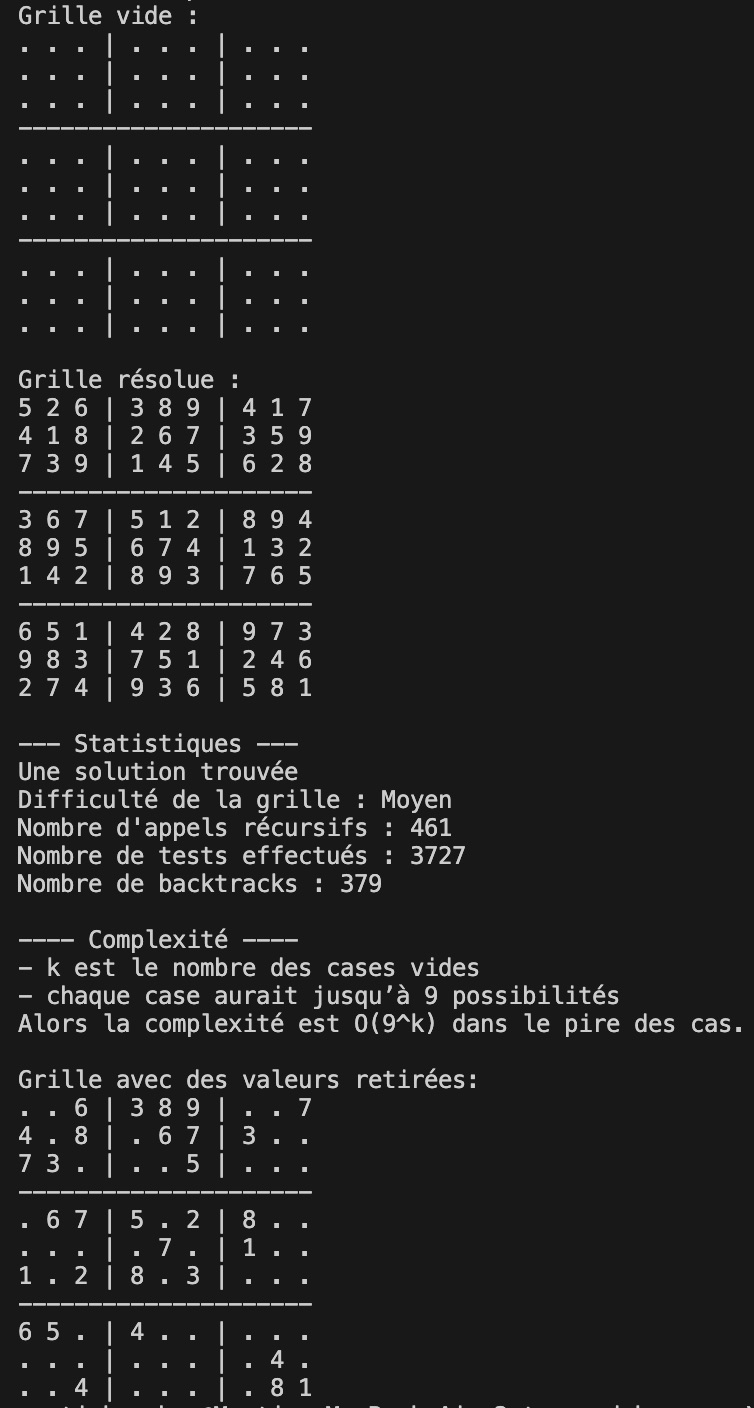
\includegraphics[width=.3\textwidth]{Terminal1.jpeg}
  \caption{Schéma de l'architecture pour le debut du projet}
\end{figure}

\vspace{4em}

\textbf{Interface Console:}\\[0.5em]

% Menu principal + choix de difficulté + grille prête
\begin{figure}[H]
  \centering
  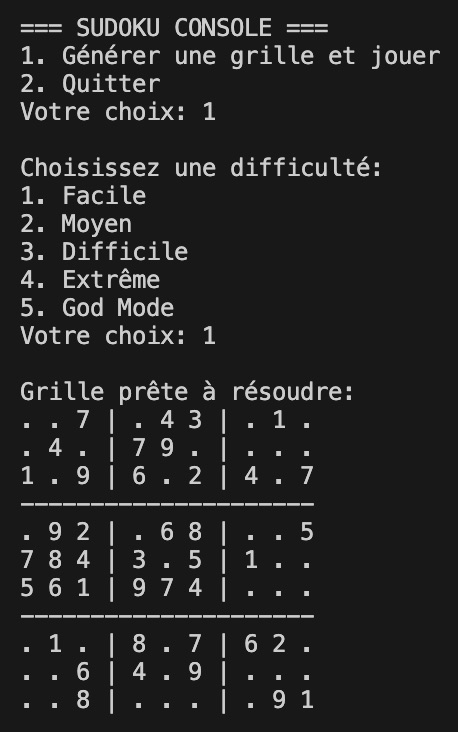
\includegraphics[width=.5\textwidth]{sudokuConsole.jpeg}
  \caption{Menu principal en console, choix de la difficulté et affichage d'une grille prête à être résolue}
\end{figure}

% Valeur invalide vs case déjà remplie (côte à côte)
\begin{figure}[H]
  \centering
  \begin{subfigure}{.48\textwidth}
    \centering
    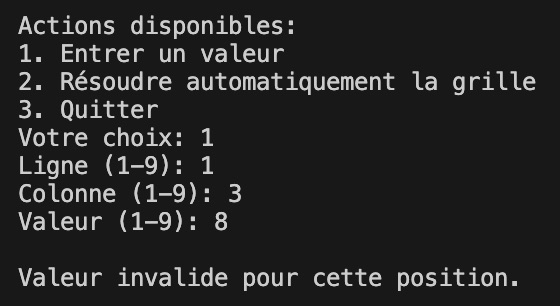
\includegraphics[width=\linewidth]{valeurInvalide.jpeg}
    \caption{Message d'erreur lors de la saisie d'une valeur invalide pour la case choisie}
  \end{subfigure}
  \hfill
  \begin{subfigure}{.48\textwidth}
    \centering
    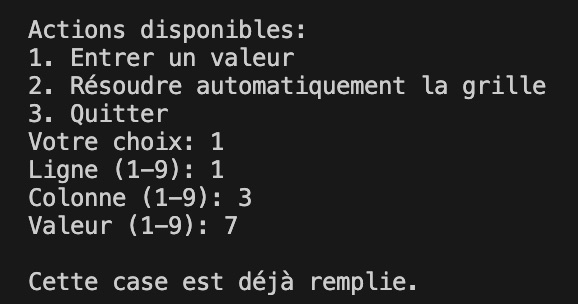
\includegraphics[width=\linewidth]{caseRemplit.jpeg}
    \caption{Message indiquant que la case sélectionnée est déjà remplie}
  \end{subfigure}
\end{figure}

% Valeur insérée + grille résolue (côte à côte)
\begin{figure}[H]
  \centering
  \begin{subfigure}{.48\textwidth}
    \centering
    
\includegraphics[width=\linewidth]{valInserer.jpeg}
    \caption{Insertion réussie d'une valeur dans la grille et mise à jour de l'affichage}
  \end{subfigure}
  \hfill
  \begin{subfigure}{.48\textwidth}
    \centering
    
\includegraphics[width=\linewidth]{grilleResolue.jpeg}
    \caption{Résolution automatique complète de la grille}
  \end{subfigure}
\end{figure}

\vspace{1em}

% ===== 4. Organisation interne du groupe =====
\section*{4. Organisation interne du groupe}
\subsection*{Répartition des rôles}
\begin{itemize}
  \item \textbf{KONCHEV Martin :} Algorithmes pour la génération de grilles et le solveur Sudoku (backtrack); Statistiques et complexité; Interface console; Rapport.
  \item \textbf{BRIOT-AMADIUE Kellyan :} (les algorithmes pour faire un parseur) (ajouter la rôle)
  \item \textbf{BARRE-GUEROT Ilan :} (ajouter la rôle).
  \item \textbf{DOLO Abdourahamane-Abdoul :} (ajouter la rôle).
\end{itemize}

\subsection*{Outils utilisés}
\begin{itemize}
  \item Git (workflow, branches, revues) : https://gitlab.etu.umontpellier.fr/e20230012387/ter-sudoku-groupX.git
  \item Communication : Discord, réunions chaque semaine.
\end{itemize}

% ===== 5. Planning prévisionnel =====
\section*{5. Planning prévisionnel}
\subsection*{Découpage en étapes / jalons}
\begin{itemize}
\item Sprint 1
\item Fin Janvier
\item Fin Fevrier
\item Fin Mars
\item Fin Avril
\end{itemize}

\subsection*{Priorités des premiers sprints}
\textbf{Sprint 1 : Analyse du problème, recherche d’algorithmes, premières implémentations.}
\begin{itemize}
  \item compteur backtrack (nombre de calculs) pour avoir la solution: le nombre de backtrack peut donner une idée de la difficulté de la grille
  \item calculer la complexité théorique de l’algorithme de résolution
  \item générer une grille complète aléatoirement
  \item faire une première interface (debug, step by step) : préparer le futur, préparation pour pouvoir afficher la prochaine étape
  \item parseur de fichier : dossier avec fichiers spéciaux où on transforme des nombres en grille
  \item chaque grille générée doit avoir une solution unique
\end{itemize}

\subsection*{Tâches jusqu’au 30 avril (Gantt prévisionnel)}
\textbf{Fin Janvier:}

Implémentation de techniques de résolution humaine
\begin{itemize}
  \item Singleton (une seule possibilité)
  \item Singleton Caché\\
\end{itemize}

\textbf{Fin Fevrier:}

Implémentation de techniques de résolution humaine
\begin{itemize}
  \item Paire cachée
  \item Triplet caché\\
\end{itemize}

\textbf{Fin Mars:}

Analyses:
\begin{itemize}
  \item Comparaison difficulté des techniques avec complexité machine entre backtrack et résolution humaine\\
\end{itemize}

\textbf{Fin Avril:}
\begin{itemize}
  \item Rédaction du rapport final
  \item Préparation de la soutenance (démonstration, présentation orale)
\end{itemize}

% ===== 6. Prototype réalisé =====
\section*{6. Prototype réalisé}
\subsection*{Description de ce qui a été testé / mis en place (même minimal)}
\emph{À compléter :} démo du plus petit incrément fonctionnel.

\subsection*{Justification des choix initiaux}
\begin{itemize}
  \item \emph{À compléter :} Choix d’algorithmes / structures de données.
  \item \emph{À compléter :} Compromis (simplicité vs performance).
\end{itemize}

\end{document}
